
%%%%%%%%%%%%%%%%%%%%%%%%%%%%%%%%%%%%%%%%%%%%%%%%%%%%%%%%%%%%%%%%%%%%%
%% This is a (brief) model paper using the achemso class
%% The document class accepts keyval options, which should include
%% the target journal and optionally the manuscript type.
%%%%%%%%%%%%%%%%%%%%%%%%%%%%%%%%%%%%%%%%%%%%%%%%%%%%%%%%%%%%%%%%%%%%%
\documentclass[journal=jacsat,manuscript=article,layout=singlecolumn]{achemso}

%%%%%%%%%%%%%%%%%%%%%%%%%%%%%%%%%%%%%%%%%%%%%%%%%%%%%%%%%%%%%%%%%%%%%
%% Place any additional packages needed here.  Only include packages
%% which are essential, to avoid problems later.
%%%%%%%%%%%%%%%%%%%%%%%%%%%%%%%%%%%%%%%%%%%%%%%%%%%%%%%%%%%%%%%%%%%%%
\usepackage{chemformula} % Formula subscripts using \ch{}
\usepackage[T1]{fontenc} % Use modern font encodings
\usepackage{epstopdf}
\usepackage{multirow}
\usepackage{adjustbox}
\usepackage{float}
\usepackage{placeins}
\usepackage{easy-todo}
\usepackage{verbatim}
%%%%%%%%%%%%%%%%%%%%%%%%%%%%%%%%%%%%%%%%%%%%%%%%%%%%%%%%%%%%%%%%%%%%%
%% If issues arise when submitting your manuscript, you may want to
%% un-comment the next line.  This provides information on the
%% version of every file you have used.
%%%%%%%%%%%%%%%%%%%%%%%%%%%%%%%%%%%%%%%%%%%%%%%%%%%%%%%%%%%%%%%%%%%%%
%%\listfiles

%%%%%%%%%%%%%%%%%%%%%%%%%%%%%%%%%%%%%%%%%%%%%%%%%%%%%%%%%%%%%%%%%%%%%
%% Place any additional macros here.  Please use \newcommand* where
%% possible, and avoid layout-changing macros (which are not used
%% when typesetting).
%%%%%%%%%%%%%%%%%%%%%%%%%%%%%%%%%%%%%%%%%%%%%%%%%%%%%%%%%%%%%%%%%%%%%
\newcommand*\mycommand[1]{\texttt{\emph{#1}}}

%%%%%%%%%%%%%%%%%%%%%%%%%%%%%%%%%%%%%%%%%%%%%%%%%%%%%%%%%%%%%%%%%%%%%
%% Meta-data block
%% ---------------
%% Each author should be given as a separate \author command.
%%
%% Corresponding authors should have an e-mail given after the author
%% name as an \email command. Phone and fax numbers can be given
%% using \phone and \fax, respectively; this information is optional.
%%
%% The affiliation of authors is given after the authors; each
%% \affiliation command applies to all preceding authors not already
%% assigned an affiliation.
%%
%% The affiliation takes an option argument for the short name.  This
%% will typically be something like "University of Somewhere".
%%
%% The \altaffiliation macro should be used for new address, etc.
%% On the other hand, \alsoaffiliation is used on a per author basis
%% when authors are associated with multiple institutions.
%%%%%%%%%%%%%%%%%%%%%%%%%%%%%%%%%%%%%%%%%%%%%%%%%%%%%%%%%%%%%%%%%%%%%

\author{Batuhan Kav}
\author{Hanne Antila}
\affiliation{Forschungszentrum Juelich, Germany}
\email{batuhankav@gmail.com}
\author{O. H. Samuli Ollila}
\author{Markus S. Miettinen}
%%%%%%%%%%%%%%%%%%%%%%%%%%%%%%%%%%%%%%%%%%%%%%%%%%%%%%%%%%%%%%%%%%%%%
%% The document title should be given as usual. Some journals require
%% a running title from the author: this should be supplied as an
%% optional argument to \title.
%%%%%%%%%%%%%%%%%%%%%%%%%%%%%%%%%%%%%%%%%%%%%%%%%%%%%%%%%%%%%%%%%%%%%
%\title[An \textsf{achemso} demo]
%  {A demonstration of the \textsf{achemso} \LaTeX\
%   class\footnote{A footnote for the title}}
\title{NMRLipids VI: Polarizable Force Fields}

%%%%%%%%%%%%%%%%%%%%%%%%%%%%%%%%%%%%%%%%%%%%%%%%%%%%%%%%%%%%%%%%%%%%%
%% Some journals require a list of abbreviations or keywords to be
%% supplied. These should be set up here, and will be printed after
%% the title and author information, if needed.
%%%%%%%%%%%%%%%%%%%%%%%%%%%%%%%%%%%%%%%%%%%%%%%%%%%%%%%%%%%%%%%%%%%%%
%\abbreviations{IR,NMR,UV}
%\keywords{American Chemical Society, \LaTeX}

%%%%%%%%%%%%%%%%%%%%%%%%%%%%%%%%%%%%%%%%%%%%%%%%%%%%%%%%%%%%%%%%%%%%%
%% The manuscript does not need to include \maketitle, which is
%% executed automatically.
%%%%%%%%%%%%%%%%%%%%%%%%%%%%%%%%%%%%%%%%%%%%%%%%%%%%%%%%%%%%%%%%%%%%%
\begin{document}

%%%%%%%%%%%%%%%%%%%%%%%%%%%%%%%%%%%%%%%%%%%%%%%%%%%%%%%%%%%%%%%%%%%%%
%% The "tocentry" environment can be used to create an entry for the
%% graphical table of contents. It is given here as some journals
%% require that it is printed as part of the abstract page. It will
%% be automatically moved as appropriate.
%%%%%%%%%%%%%%%%%%%%%%%%%%%%%%%%%%%%%%%%%%%%%%%%%%%%%%%%%%%%%%%%%%%%%
%\begin{tocentry}

%\end{tocentry}

%%%%%%%%%%%%%%%%%%%%%%%%%%%%%%%%%%%%%%%%%%%%%%%%%%%%%%%%%%%%%%%%%%%%%
%% The abstract environment will automatically gobble the contents
%% if an abstract is not used by the target journal.
%%%%%%%%%%%%%%%%%%%%%%%%%%%%%%%%%%%%%%%%%%%%%%%%%%%%%%%%%%%%%%%%%%%%%
\begin{abstract}
	
	For the initial project description, please refer to \\ https://github.com/batukav/NMRlipidsVIpolarizableFFs/blob/master/Manuscript/manuscript.pdf
	
\end{abstract}

%%%%%%%%%%%%%%%%%%%%%%%%%%%%%%%%%%%%%%%%%%%%%%%%%%%%%%%%%%%%%%%%%%%%%
%% Start the main part of the manuscript here.
%%%%%%%%%%%%%%%%%%%%%%%%%%%%%%%%%%%%%%%%%%%%%%%%%%%%%%%%%%%%%%%%%%%%%
\section{Introduction}
Conventional classical molecular dynamics (MD) simulations only consider electrostatics as interactions between static point charges, set by molecular dynamics models (force fields) as an input in the beginning of the simulation. The dynamic effects arising from polarizability are ignored or at most enter the simulations in an averaged fashion in the force field parametrization process. However, since decades work has been underway to make MD simulations explicitly polarizable in the hopes of reaching a more accurate description of the system. In the case of biomembranes (lipid bilayers), spesifically, including polarizability the molecular (dielectric) environment varies dramatically while crossing the membrane from the water phase across the dipolar/charged headgroup interface to the hydrophobic tail region and including explicit polarizability has the potential to provide more accurate description of membrane binding, membrane crossing, and behaviour and interactions of molecules residing within membranes, such as membrane protein folding. There certainly is room for improvement: efforts from the NMRlipids opens science community have showed that the current classical lipid models cannot correctly reproduce the conformational ensemble~\cite{}, conformational dynamics~\cite{}, or ion biding~\cite{} within the simulations. 

Historically, there has been three main approaches to modelling polarizability: 1) the induced point dipole/multipole model where polarizable point dipoles are placed on chosen sites on a molecule, 2) the classical Drude oscillator model where polarization is modelled by separating a core and a shell charge with a spring which stretches according to the enviroment giving the site a dipole moment, and 3) electronegativity equilization (fluctuating charge) model where atomic charges are no longer constant but can change according to the electronegativities of the molecule atoms and the electric fields from the molecular enviroment. In recent years the first two have surpassed the third in popularity. However, all of these approaches result in an increasing computational cost, e.g, by introducing new types of interactions, more interactions sites, or by requiring a shorter time step in the simulations.


%To avoid polarizability catastrophe where two closeby polarizable sites feed off from each other and the dipole moments grow infinitely



Considering the increasing popularity of both implicitly and explicitly polarizable force fields and the increased computational computational cost that they require, systematic benchmark study polarizable force field quality is in high need. A few published studies reviewing the state of the polarizable force fields for biomolecules did not go beyond citing the results from the existing studies~\cite{inakollu2020polarisable,jin,baker2015polarizable}. Recent publications show that implicit inclusion of polarizability improves cation binding simulations when evaluated against NMR data~\cite{Melcr:2018a, melcr2019improved}. These results suggest that ion binding would be better captured in simulations with polarizable force fields. 
At the moment, there are three main polarizable lipid force fields with explicit electronic polarization: CHARMM-Drude~\cite{li2017drude}, AMOEBA~\cite{chu2018anionicpolarizable,chu2018polarizable}, and CHARMM-Fluctuating Charge (FQ)~\cite{lucas2012charge}. 
Here we evaluate the performance of two polarizable force fields with lipid parameters available, CHARMM-Drude~\cite{li2017drude} and AMOEBA~\cite{chu2018anionicpolarizable,chu2018polarizable}, against NMR data. We use NMR order parameters to evaluate  structural properties and cation binding, whereas NMR relaxation rates and correlation times are utilized to benchmark the lipid conformational dynamics. Furthermore, we compare the results to the non-polarizable simulations from the NMRlipids databanks.




\section{Methods}
\subsection{Practical pitfalls of polarizable biomembrane simulations}


\subsubsection{Building a polarizable force field}

The atomic point charges describing the electrostatics in non-polarizable force fields are typically parameterized by fitting to the electrostatic potential energy surface around one or few conformers obtained from ab initio calculations. One then proceeds to build on top of that the parameters for Lennard-Jones interactions and the dihedrals using a mixture of experimental (such as heats of vaporizations) and quantum mechanical information. For a polarizable force fields, this process has to be redone as in the first step the polarizable contribution has to be separated from the "static" one. Furthermore, for the polarization models considered here, an additional cutoff/damping scheme needs to be introduced to prevent polarization catastrophe---a phenomenon where close-by dipoles feed of each others and their dipole moments (and energy) grows into infinity.

Both polarizable lipid force fields considered here use a bottom up approach where parameters are first obtained for smaller molecules or molecular fragments from which the lipid models are then built.  In the CHARMM-Drude model, the polarizabilities, the Thole damping factors used to prevent polarization catastrophe, and the partial charges where determined by fitting to a discretized QM potential energy surface around the molecule. More spesifically, the pertubations of the potential energy surface in the presence of a small charge where observed to separate the dynamic polarizability contribution. They then proceeded to use enthalpies of vaporation along with QM calculations of molecular interaction enegies to obtain the Lennard-Jones parameters, and on top of that dihedral potentials were introduced to reproduce the QM potential energy profiles along a dihedral rotation. Finally, the dihedrals of the lipid head groups where refined targetting the NMR order parameters.

In the Amoeba force field, a set of atomic multipoles were first obtained based on the QM electron densities using Stone's distributed multipole analysis. The atoms were then assigned polarizabilities according to the AMOEBA atom types and   induced dipole contribution was self consistently substracted from the permanent dipoles~\cite{shi2013proteinamoeba}. The charges (monopoles) were then kept constant while the multipoles were refined against the electrostatic potential energy surface around few conformers of the molecular fragments. %Multipoles are allowed to induce only dipoles at polarizable sites outside their immediate environment (polarization group). 
After electrostatic parameters were set, the Lennard-Jones parameters were taken from previous AMOEBA parameterizations of smaller molecules containing same functional groups~\cite{Ren2011polorganic,shi2011hydration}, and then refined against molecule - water (gas phase) interaction energies. After settling all the nonbonded parameters, dihedral potentials were parameterised based on the QM conformational energy profiles.

\begin{comment}
- polarization contribution has to be separated from point charge electrostatics in the parametrization process.
- for the models considered here (Drude, IDP) one has to prevent the polarization catastrophe somehow (Thole damping parameter)
- Brief explanation how the two FFs studied here were built.

Notes on CHARMM-Drude parametrization:
- bottom up approach. Permantent charge, polarizability and screening factors from QM. Polarizability decoupled from permanent by fitting to changes in PES? 
- Non-bonded electrostatics parameters calculated based on QM.
- LJ from enthalpies of vaporization together .with QM data
- Dihedrals from QM scans for model compounds, then refined to according to the order parameters of the headgroup using re-weighted MD and an genetic algorithm.

Notes on Amoeba parametrization (this is NOT well explained in the paper)
-bottom up approach
-Stone distributed multipole analysis to get the multipoles from the QM electron densities. Divided into permanent and induced.
-Then iterative fitting to QM-PES for electrostatics
-WdW from 1) optimization to hydration energy calculations and 2) QM fragment-water gas phase calculations.
-dihedrals optimized to QM potentials
-no mention of the screening for polarization? Do they use some AMOEBA value
\end{comment}
\subsubsection{Using a polarizable force field}

The increased level of detail portrayed by explicit treatment of electronic polarizability comes with certain costs. The first cost is the increased computational complexity reduces the simulation speed. For the Drude force field, this slowdown occurs both because the addition of the Drude particles increases the number of interaction pairs and the employed extended dual-Langevin thermostat requires 1~fs integration time step. Current AMOEBA force field can use a multi time-step integration algorithm where the non-electronic interactions are iterated with a 2~fs time step whereas more computationally unstable polarization terms are iterated with a smaller time step. Yet, this usage of a multi-time step integration scheme does not overcome the slowdown resulting from the computationally demanding polarization calculations. As a result, one experiences almost a ten-fold decrease in the simulation speed while using the polarizable force fields. The second cost is due to the limited software support for both running and analyzing the simulations. Currently only OpenMM supports both AMOEBA and Drude force fields. NAMD can only run the Drude force field whereas TINKER is only valid for AMOEBA force field and it does not support semi-isotropic pressure coupling, which decouples the pressure tensor in $xy$ and $z$-direction and is crucial for correctly evaluating the ion binding properties of the bilayers (\todo{This needs a reference, I remember Samuli mentioning this during a chat}). On the other hand, GROMACS, which has been the most popular MD engine within the bilayer simulation field, does not support any polarizable force field simulations. This is particularly important, as GROMACS also comes with many built-in functions for analyzing the trajectories and many of these functions require a GROMACS tpr file and subsequently cannot be utilized for analyzing the trajectories generated by other MD engines. This hinders the researchers from using well-tested analysis tools creating an overhead during the trajectory analysis while making results more prone to error. Therefore, open-source Python libraries for trajectory analysis like MDAnalysis, MDtraj, and LiPhyphilic (based on MDAnalysis) that can work on multiple trajectory and topology formats are gaining more attention.

Thanks to its recent update, CHARMM-GUI now can generate the topology and input parameters for the Drude force field, which greatly simplifies the employment of this model.

\subsection{Simulations with CHARMM-Drude parameters}





Current versions of the polarizable force fields require "good" starting structures. To achieve this, for every system, 200~ns long MD simulations with the non-polarizable CHARMM36 force field are run. The last frames from these simulations are fed into the CHARMM-GUI Drude Prepper to generate the input structures and OpenMM run files. Each bilayer contains 36 lipids in each leaflet. Simulations are run with the OpenMM MD engine. 

The trajectories are publicly available on Zenodo.

\subsection{Simulations with AMOEBA parameters}


AMOEBA parameters are obtained from Githb [ref]. 

\subsection{Analysis of simulations}
Order parameters are calculated using the script "OrderParameters.py" under\\ "https://github.com/batukav/NMRlipidsVIpolarizableFFs/tree/master/scripts". \\
The order parameters are first calculated for each lipid as an average over time, and then averaged over the lipids. The error estimates are calculated as the standard error of the mean from the second average.
Dihedral distributions are calculated using the script "calcDihedral.py" under\\ "https://github.com/batukav/NMRlipidsVIpolarizableFFs/tree/master/scripts" .\\
The $R_{1}$ rates and effective correlation times, along with the accompanying error estimates, are quantified from the trajectories as elaborated in Ref.~\citenum{Antila2021}. In-house python script available at XXX was used for this purpose.
\subsection{Simulation Details and data availability}
This project is performed using the "NMRLipids Databank" format and all related files, except the trajectories, are available under\\ "https://github.com/batukav/NMRlipidsVIpolarizableFFs/"


% Please add the following required packages to your document preamble:
\newpage
%\begin{adjustbox}{angle=90}
\begin{table}[]
\begin{tabular}{cccccccccc}
	Lipid/counter-ions                & force field  & Ion (M) & N$_{l}$ & N$_{w}$ & N$_{ion}$ & T (K) & t$_{sim}$ (ns) & t$_{analysis}$ (ns) & files \\ \hline
POPC                              & CHARMM-Drude & NA      & NA       & 6400       & 0         & 303    & 500              & 400         &          \cite{kav_batuhan_2021_4604630}    \\ \hline
POPE                              & CHARMM-Drude & NA      & NA       & 6400       & 0         & 303    & 350              & 300         &          \cite{kav_batuhan_2021_4665773}    \\ \hline
	\multirow{4}{*}{POPC:NaCl}        & CHARMM-Drude & 0.350   & 144      & 6400     & 41         & 303   & 500             & 400                  & \cite{kav_batuhan_2020_4683386}   \\
				  & CHARMM-Drude & 0.450   & 144      & 6400     & 51         & 303   & 500             & 400                  & \cite{kav_batuhan_2020_4683398}   \\
				  & CHARMM-Drude & 0.650   & 144      & 6400     & 77         & 303   & 500             & 400                  & \cite{kav_batuhan_2020_4683405}   \\
				  & CHARMM-Drude & 1.0     & 144      & 6400     & 115        & 303   & 500             & 400                  & \cite{kav_batuhan_2020_4683411}   \\ \hline
	\multirow{3}{*}{POPC:CaCl$_{2}$} & CHARMM-Drude & 0.350   & 144      & 6400     & 41         & 303   & 500             & 400                  & \cite{kav_batuhan_2020_4683393}   \\
				  & CHARMM-Drude & 0.450   & 144      & 6400     & 52         & 303   & 500             & 400                  & \cite{kav_batuhan_2020_4683391}   \\
				  & CHARMM-Drude & 0.650   & 144      & 6400     & 76         & 303   & 500             & 400                  & \cite{kav_batuhan_2020_4683394} \\
				  & CHARMM-Drude & 1.0   & 144      & 6400     & 114         & 303   & 500             & 400                  & \cite{kav_batuhan_2021_4738966}
				  
\end{tabular}
\end{table}
%\end{adjustbox}

\section{Results}

\subsection{Evaluation of lipid bilayer properties simulated with polarizable force fields}

\todo{Batuhan: Do we want to have a table showing the area per lipid, volume per lipid etc. type of values from these simulations?}
%\begin{figure}[!hbt]
%	\centering
%	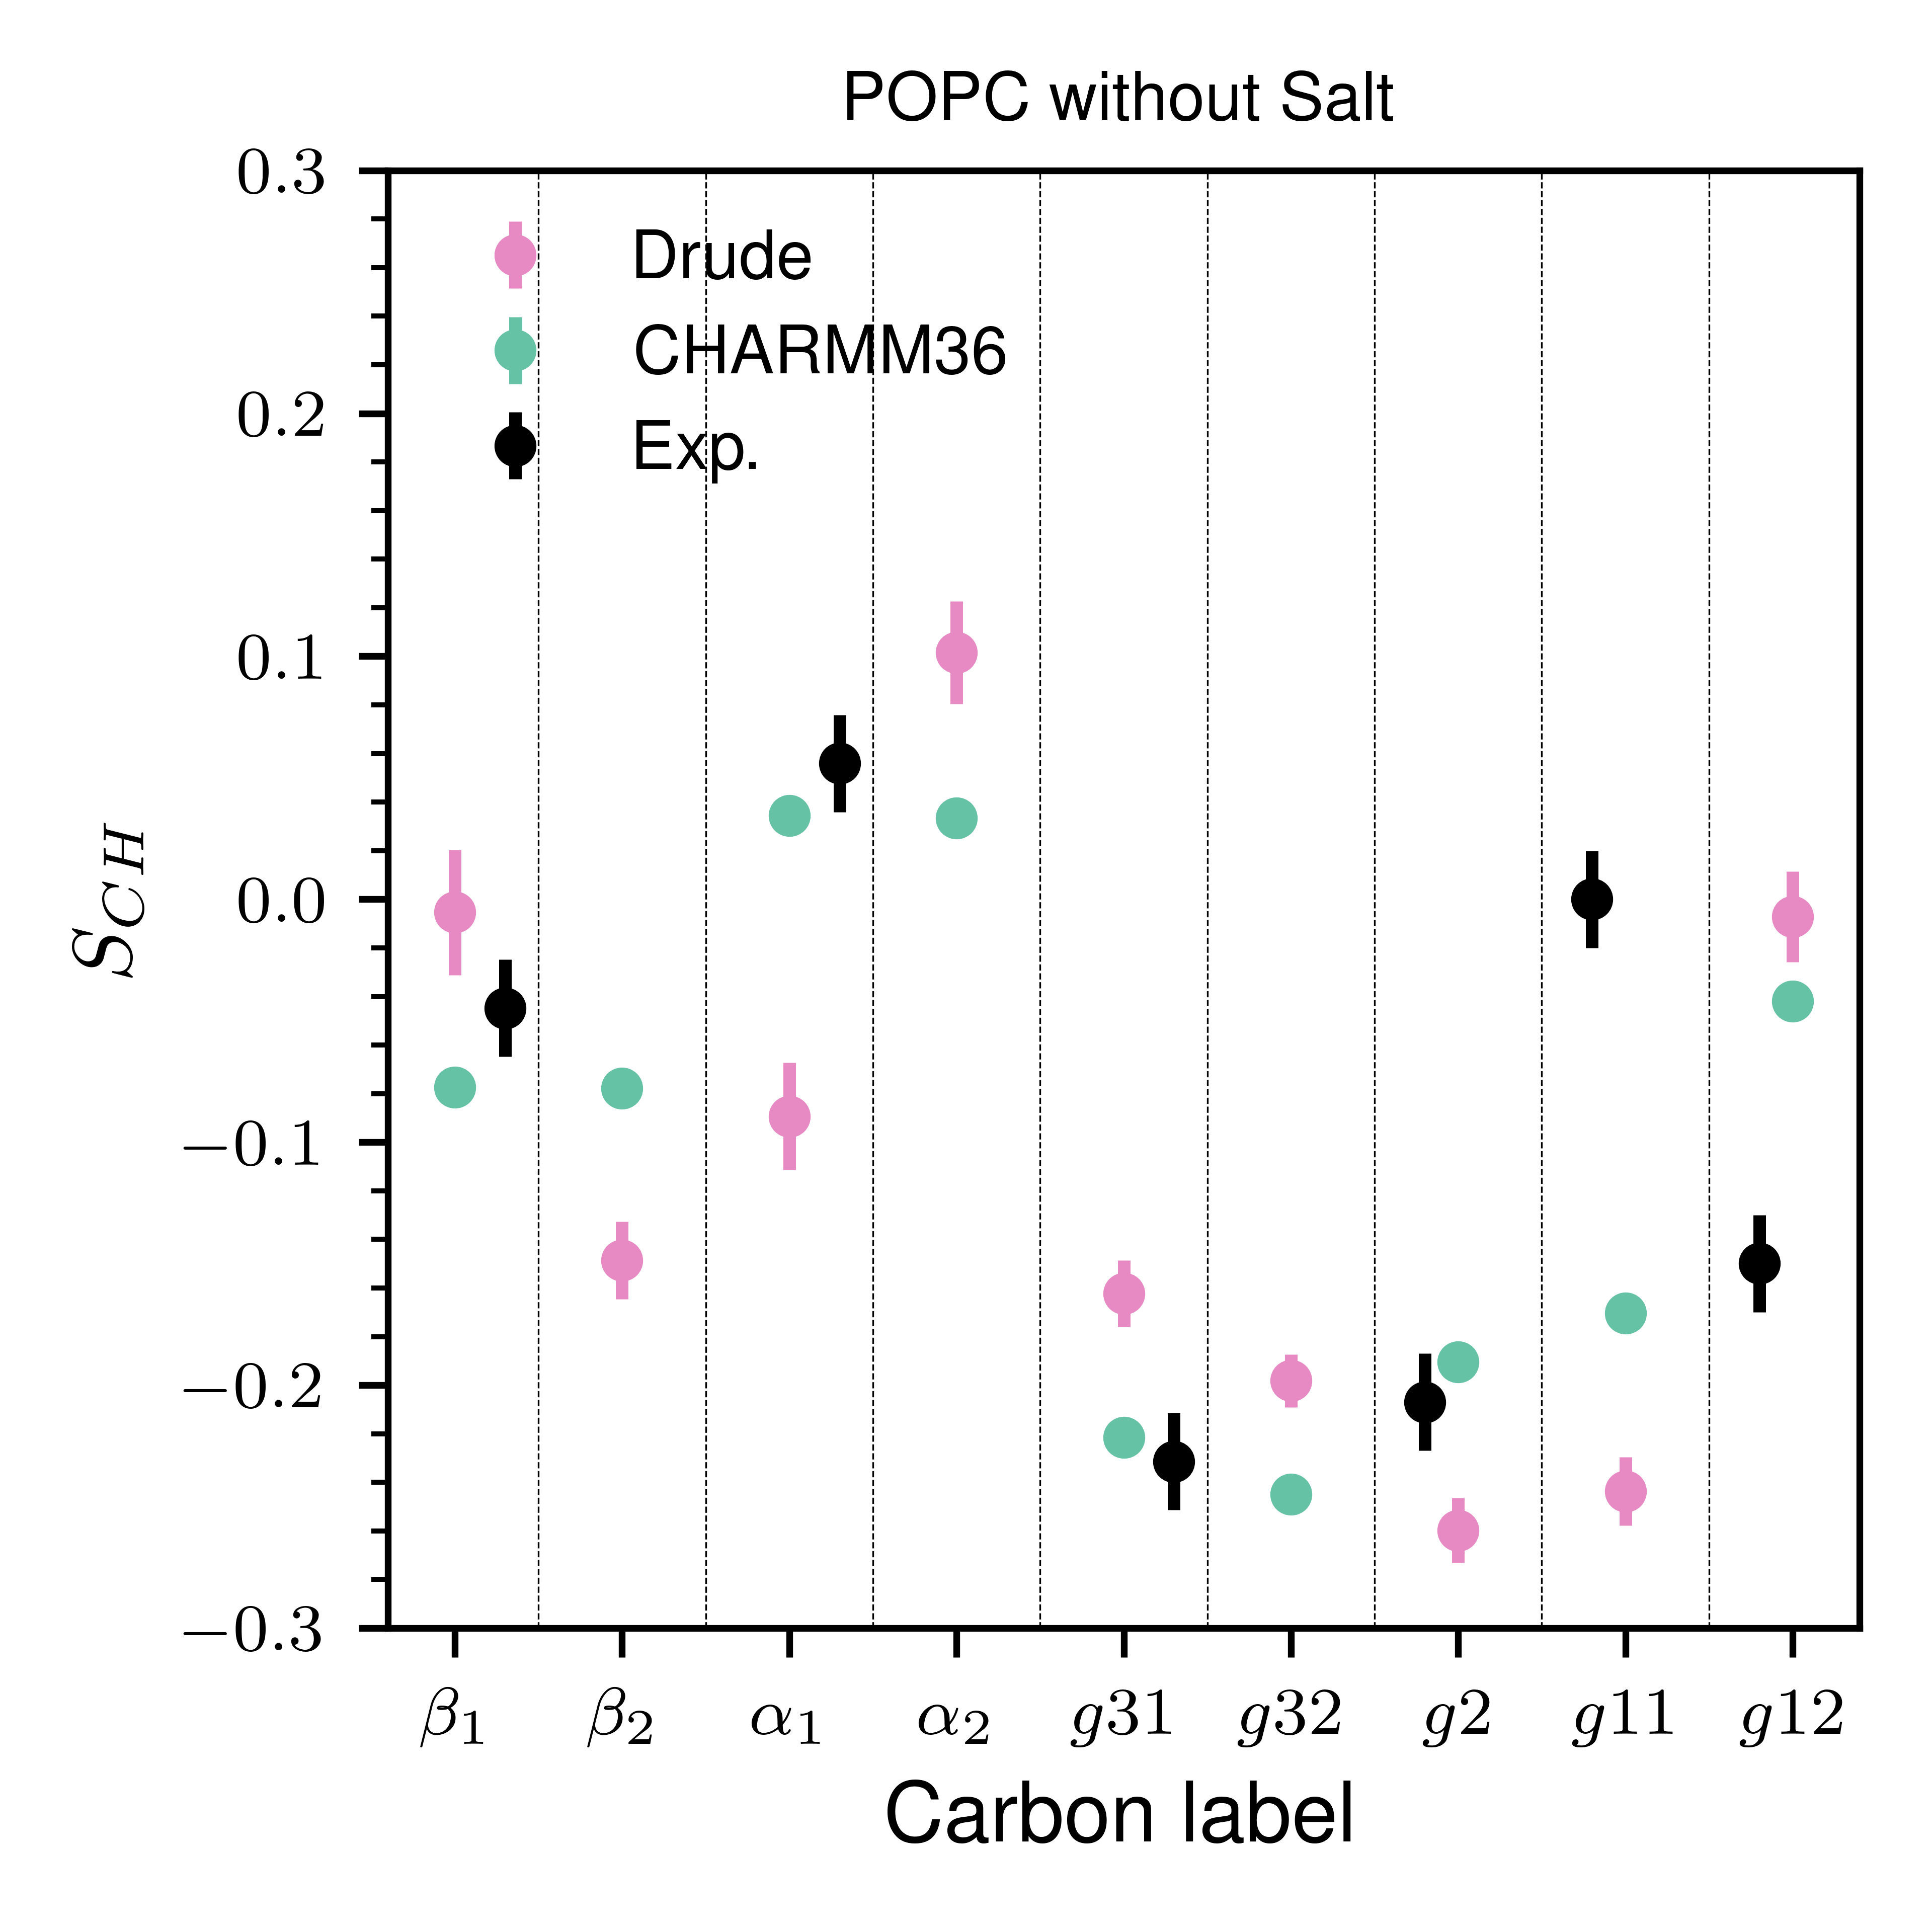
\includegraphics{popc_order_parameters_nosalt.png}
%	\caption{The head group and glycerol backbone order parameters $S_{CH}$ for the POPC simulations without salt.}
%	\label{fig:popc_order_no_salt}
%        \todo{SAMULI: It would be good to put the experimental value also to second hydrogen even though it would be the same as for first.
%          Now it looks like that those values would not be known.} \\
%        \todo{SAMULI: y-axis should be more zoomed in.} \\
%        \todo{SAMULI: Similar figure for POPE (now figure 4) could be here as panel B).}
%\end{figure}

%\begin{figure}[!hbt]
%	\centering
%	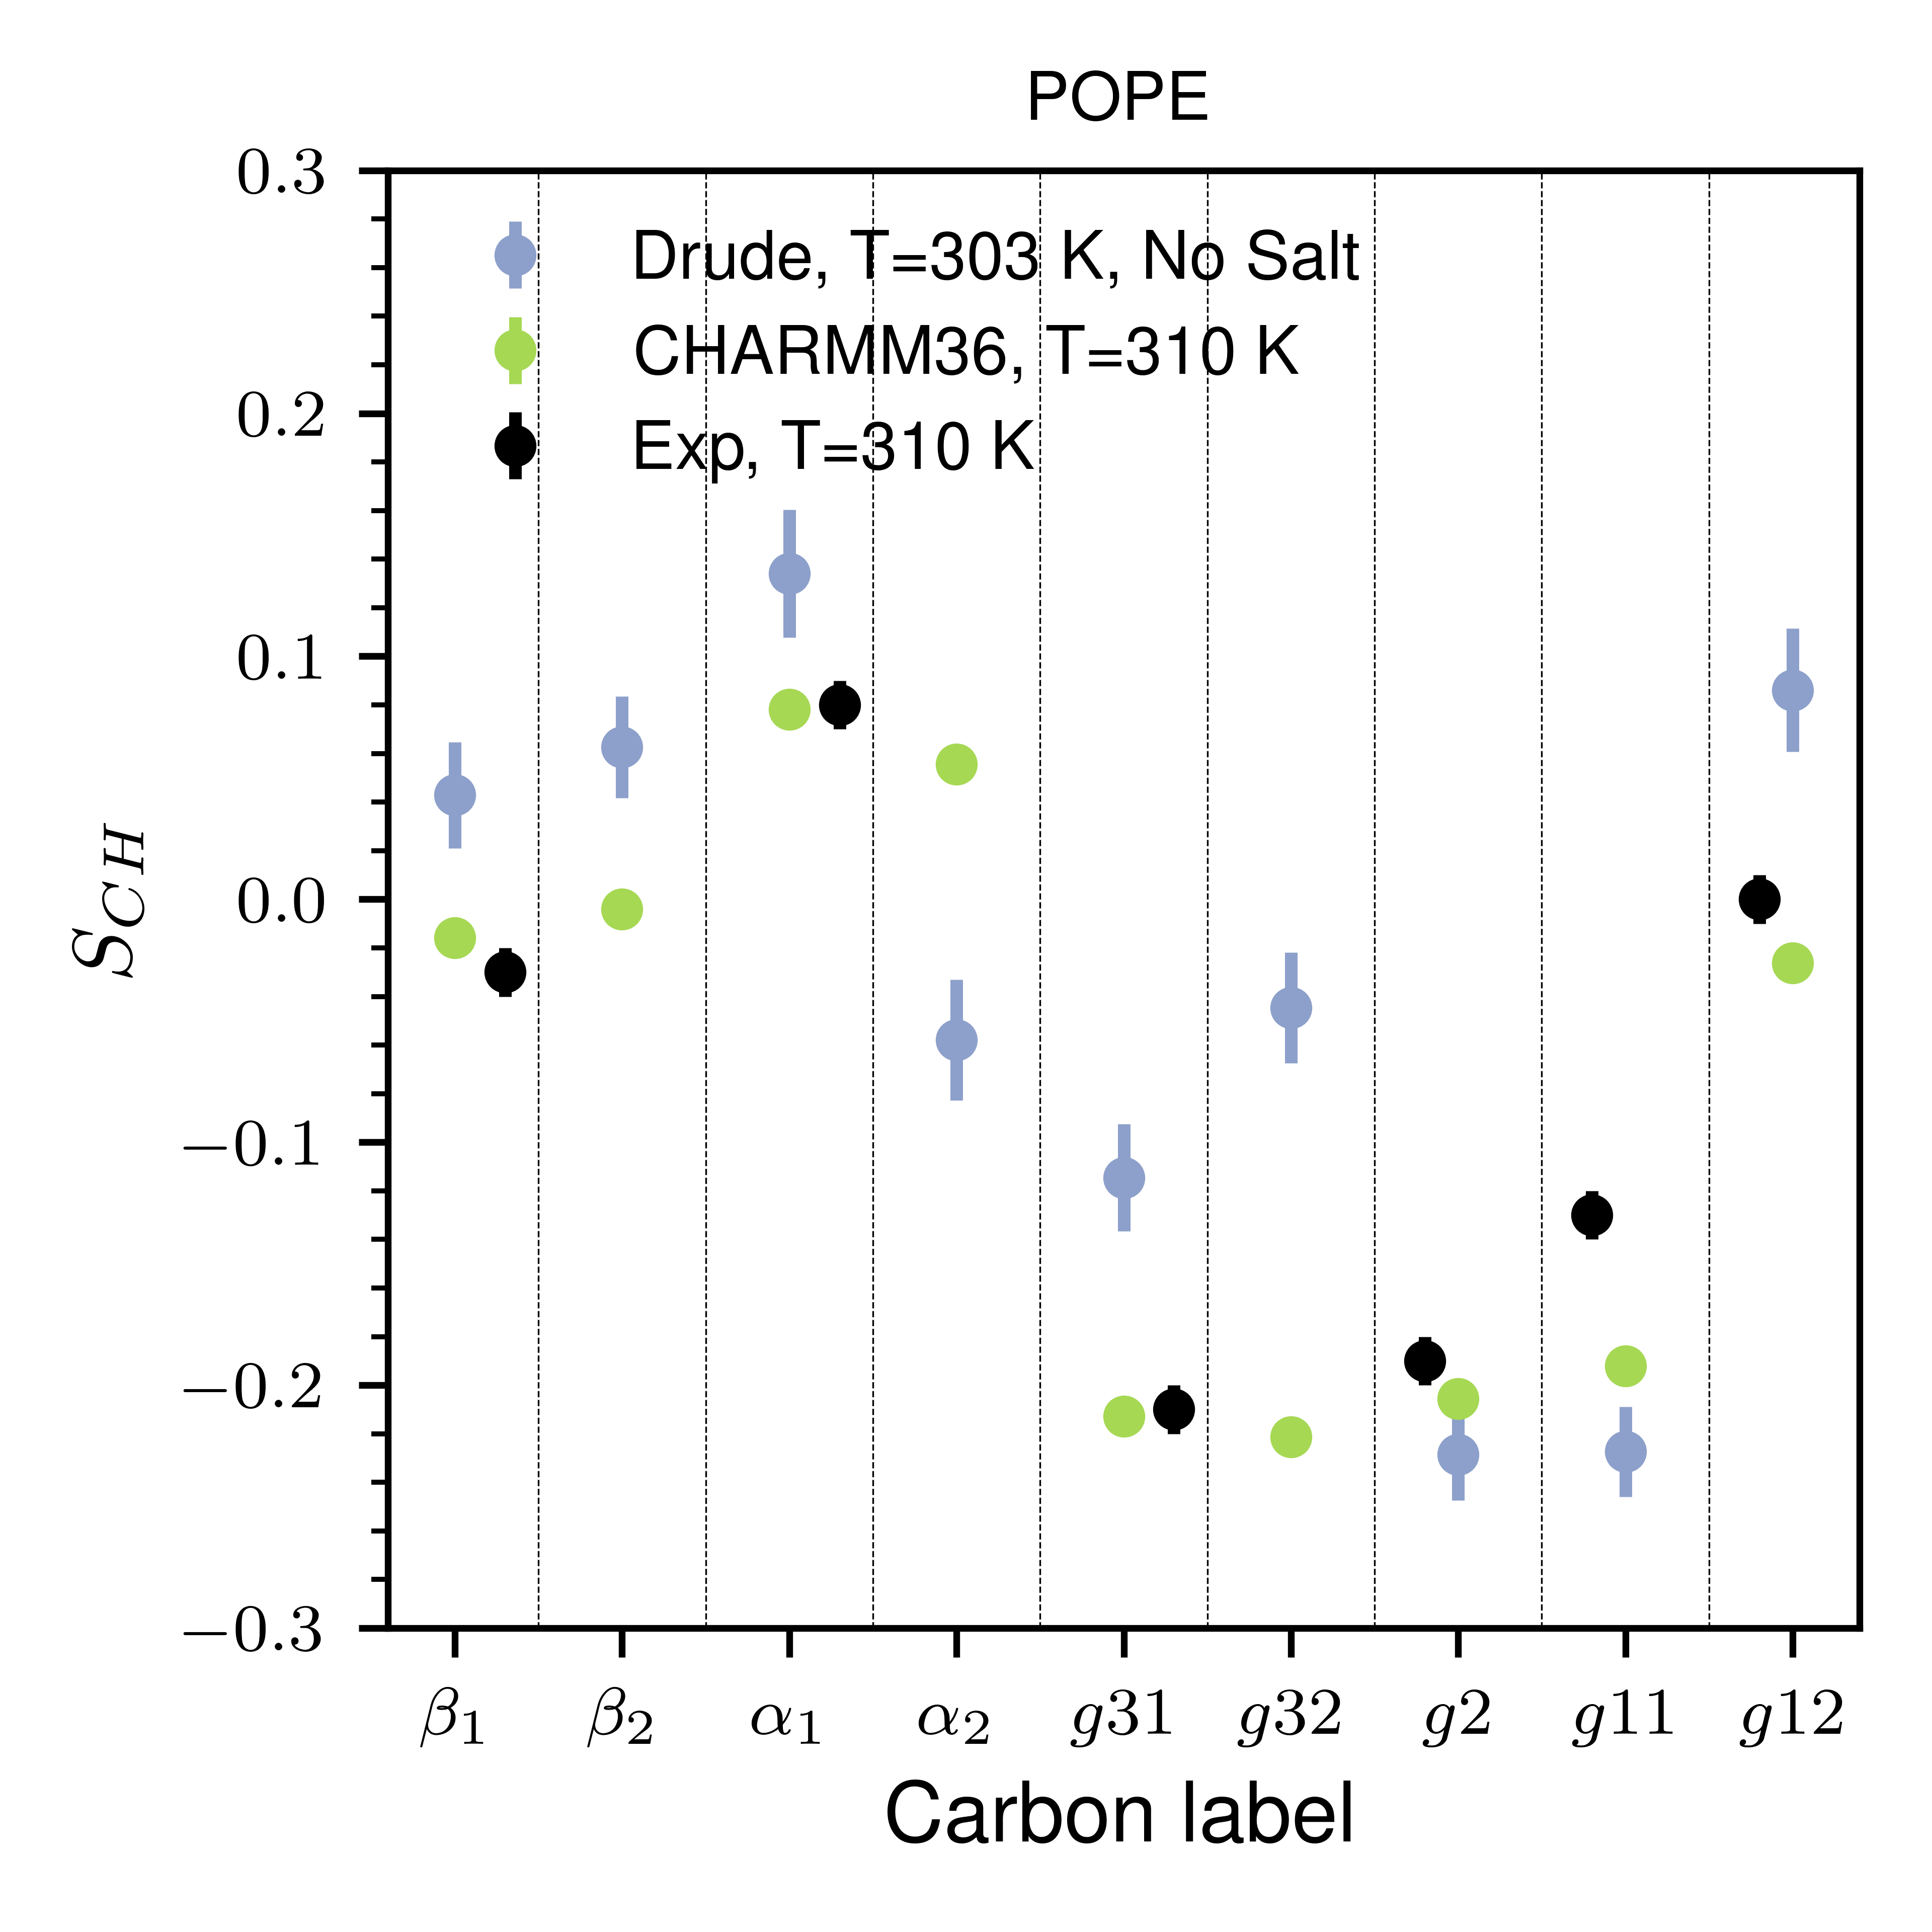
\includegraphics{pope_order_parameters.png}
%	\caption{The head group and glycerol backbone order parameters $S_{CH}$ for the POPE simulations.}
%	\label{fig:pope_order}
%        \todo{SAMULI: Move to panel B) in Figure 1.} \\
%        \todo{SAMULI: y-axis should be more zoomed in.} 
%\end{figure}

\begin{figure}[!hbt]
    \centering
    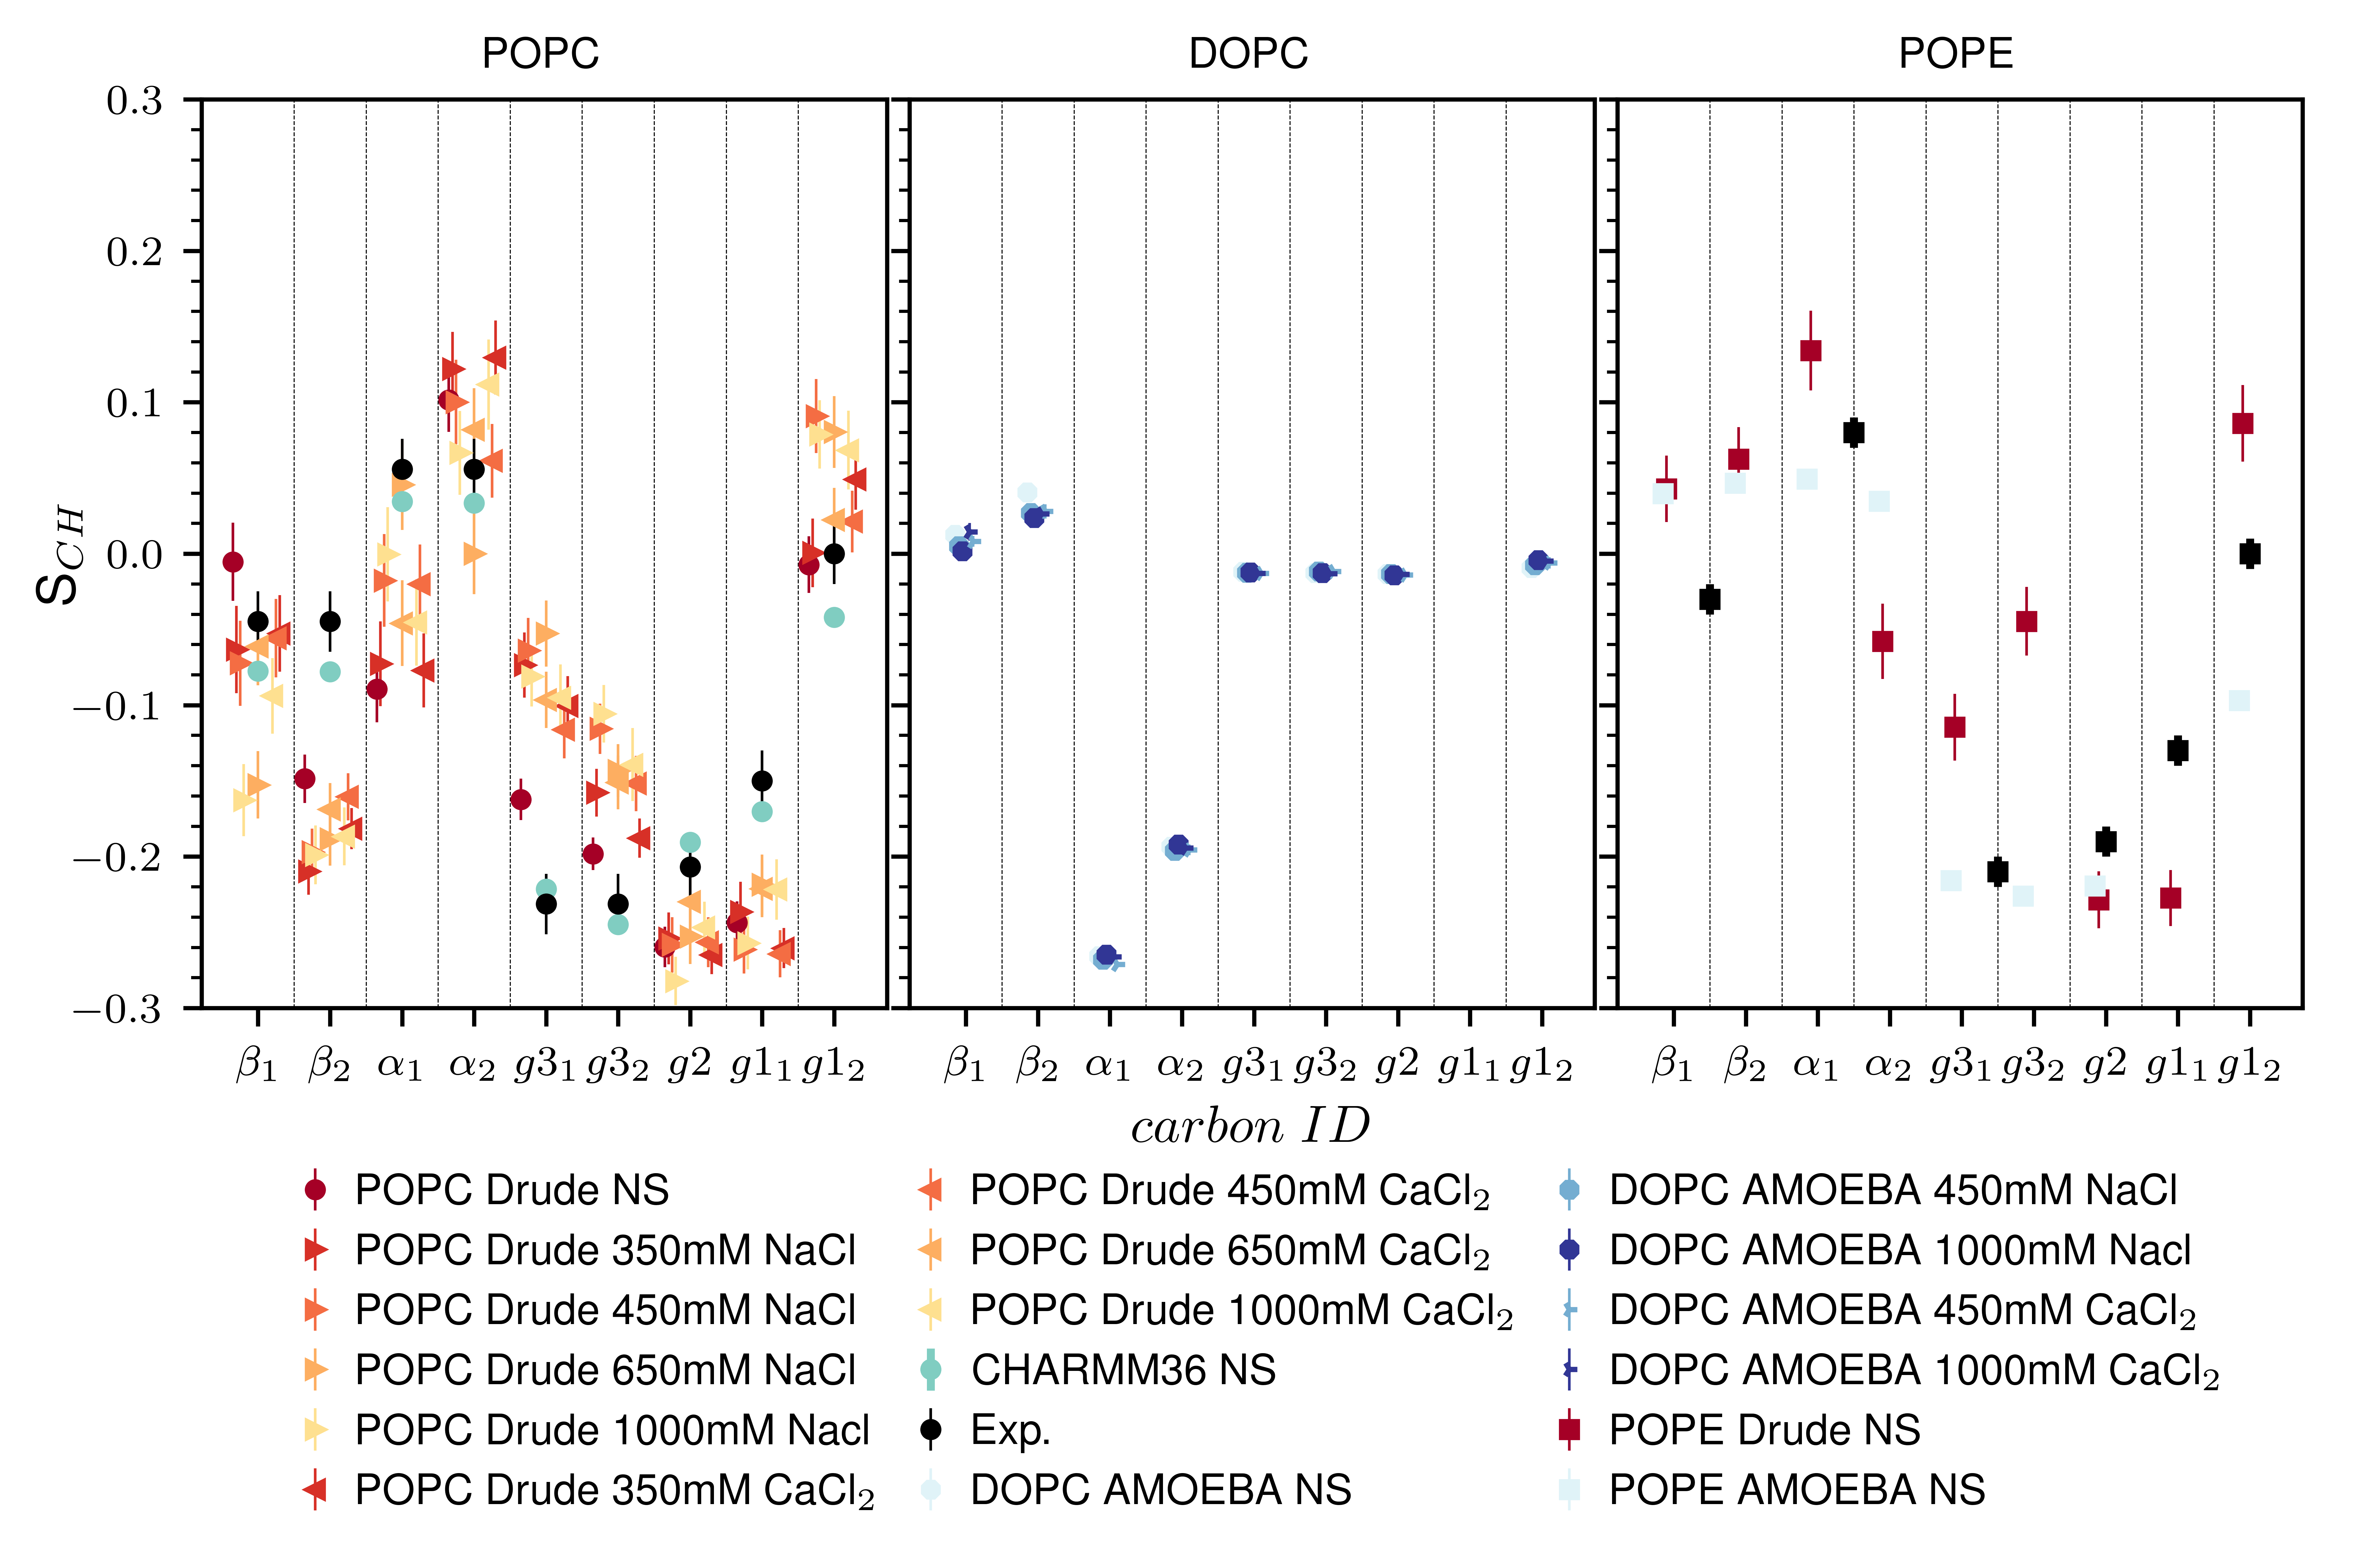
\includegraphics{Figures/order_parameters.png}
    \caption{Order parameters calculated from the simulations}
    \label{fig:order_parameters}
    \todo{Batuhan: Exp for DOPC?}
    \todo{Batuhan: Charmm or any other simulation data for DOPC?}
\end{figure}

%\begin{figure}[!hbt]
%	\centering
%	\includegraphics{dihedral_distributions_for_all.png}
%	\caption{The distributions of the torsion angles for the head group atoms}
%	\label{fig:dihedral}
%        \todo{SAMULI: I am not sure if we need this figure at all.
%          Or were you planning to discuss why order parameter response to ions is qualitatively incorrect in Drude PC?
%          If yes, then maybe remove POPE from this figure.
%        }
%\end{figure}

\begin{figure}[!hbt]
	\centering
	\includegraphics{Figures/dihedral_distributions_no_salt.png}
	\caption{The distributions of the torsion angles for the head group atoms without the presence of salt.}
	\label{fig:dihedral_no_salt}
        \todo{SAMULI: I am not sure if I see POPE CHARMM36 lines in this figure.
          Also, colors, lines styles and/or widths could be better used to distinguish common and different elements in each line.
        For example, CHARMM36 with thick lines, drude thin lines, POPC black, POPE red, or something like that.}
        \todo{Batuhan: I'll fix the color scheme, add amoeba results, and move it to the SI section}
\end{figure}

\begin{figure}[!hbt]
	\centering
	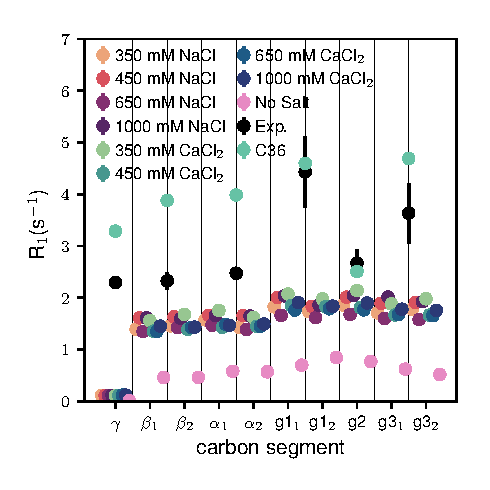
\includegraphics{Figures/correlation_times.eps}
	\caption{R1 times calculated for the POPC system. Experimental values are obtained from Ref.~\cite{antila2020quasi}}
	\label{fig:correlation_times}
        \todo{SAMULI: Are ''No Salt'' and all ion containing systems from Drude? Is it really true that addition of any salt increases the
        values to the same independently on the amount?}
        \todo{HANNE: are you going to add the teffs? You got the lower limit out of them right? Or maybe we can just mention that the correlation times were super slow which compounds to the already heavy computational load (one needs to simulate even longer to get convergence) }
\end{figure}

\clearpage

\subsection{Ion binding to membranes in simulations with polarizable force fields}

%\begin{figure}[!hbt]
%	\centering
%	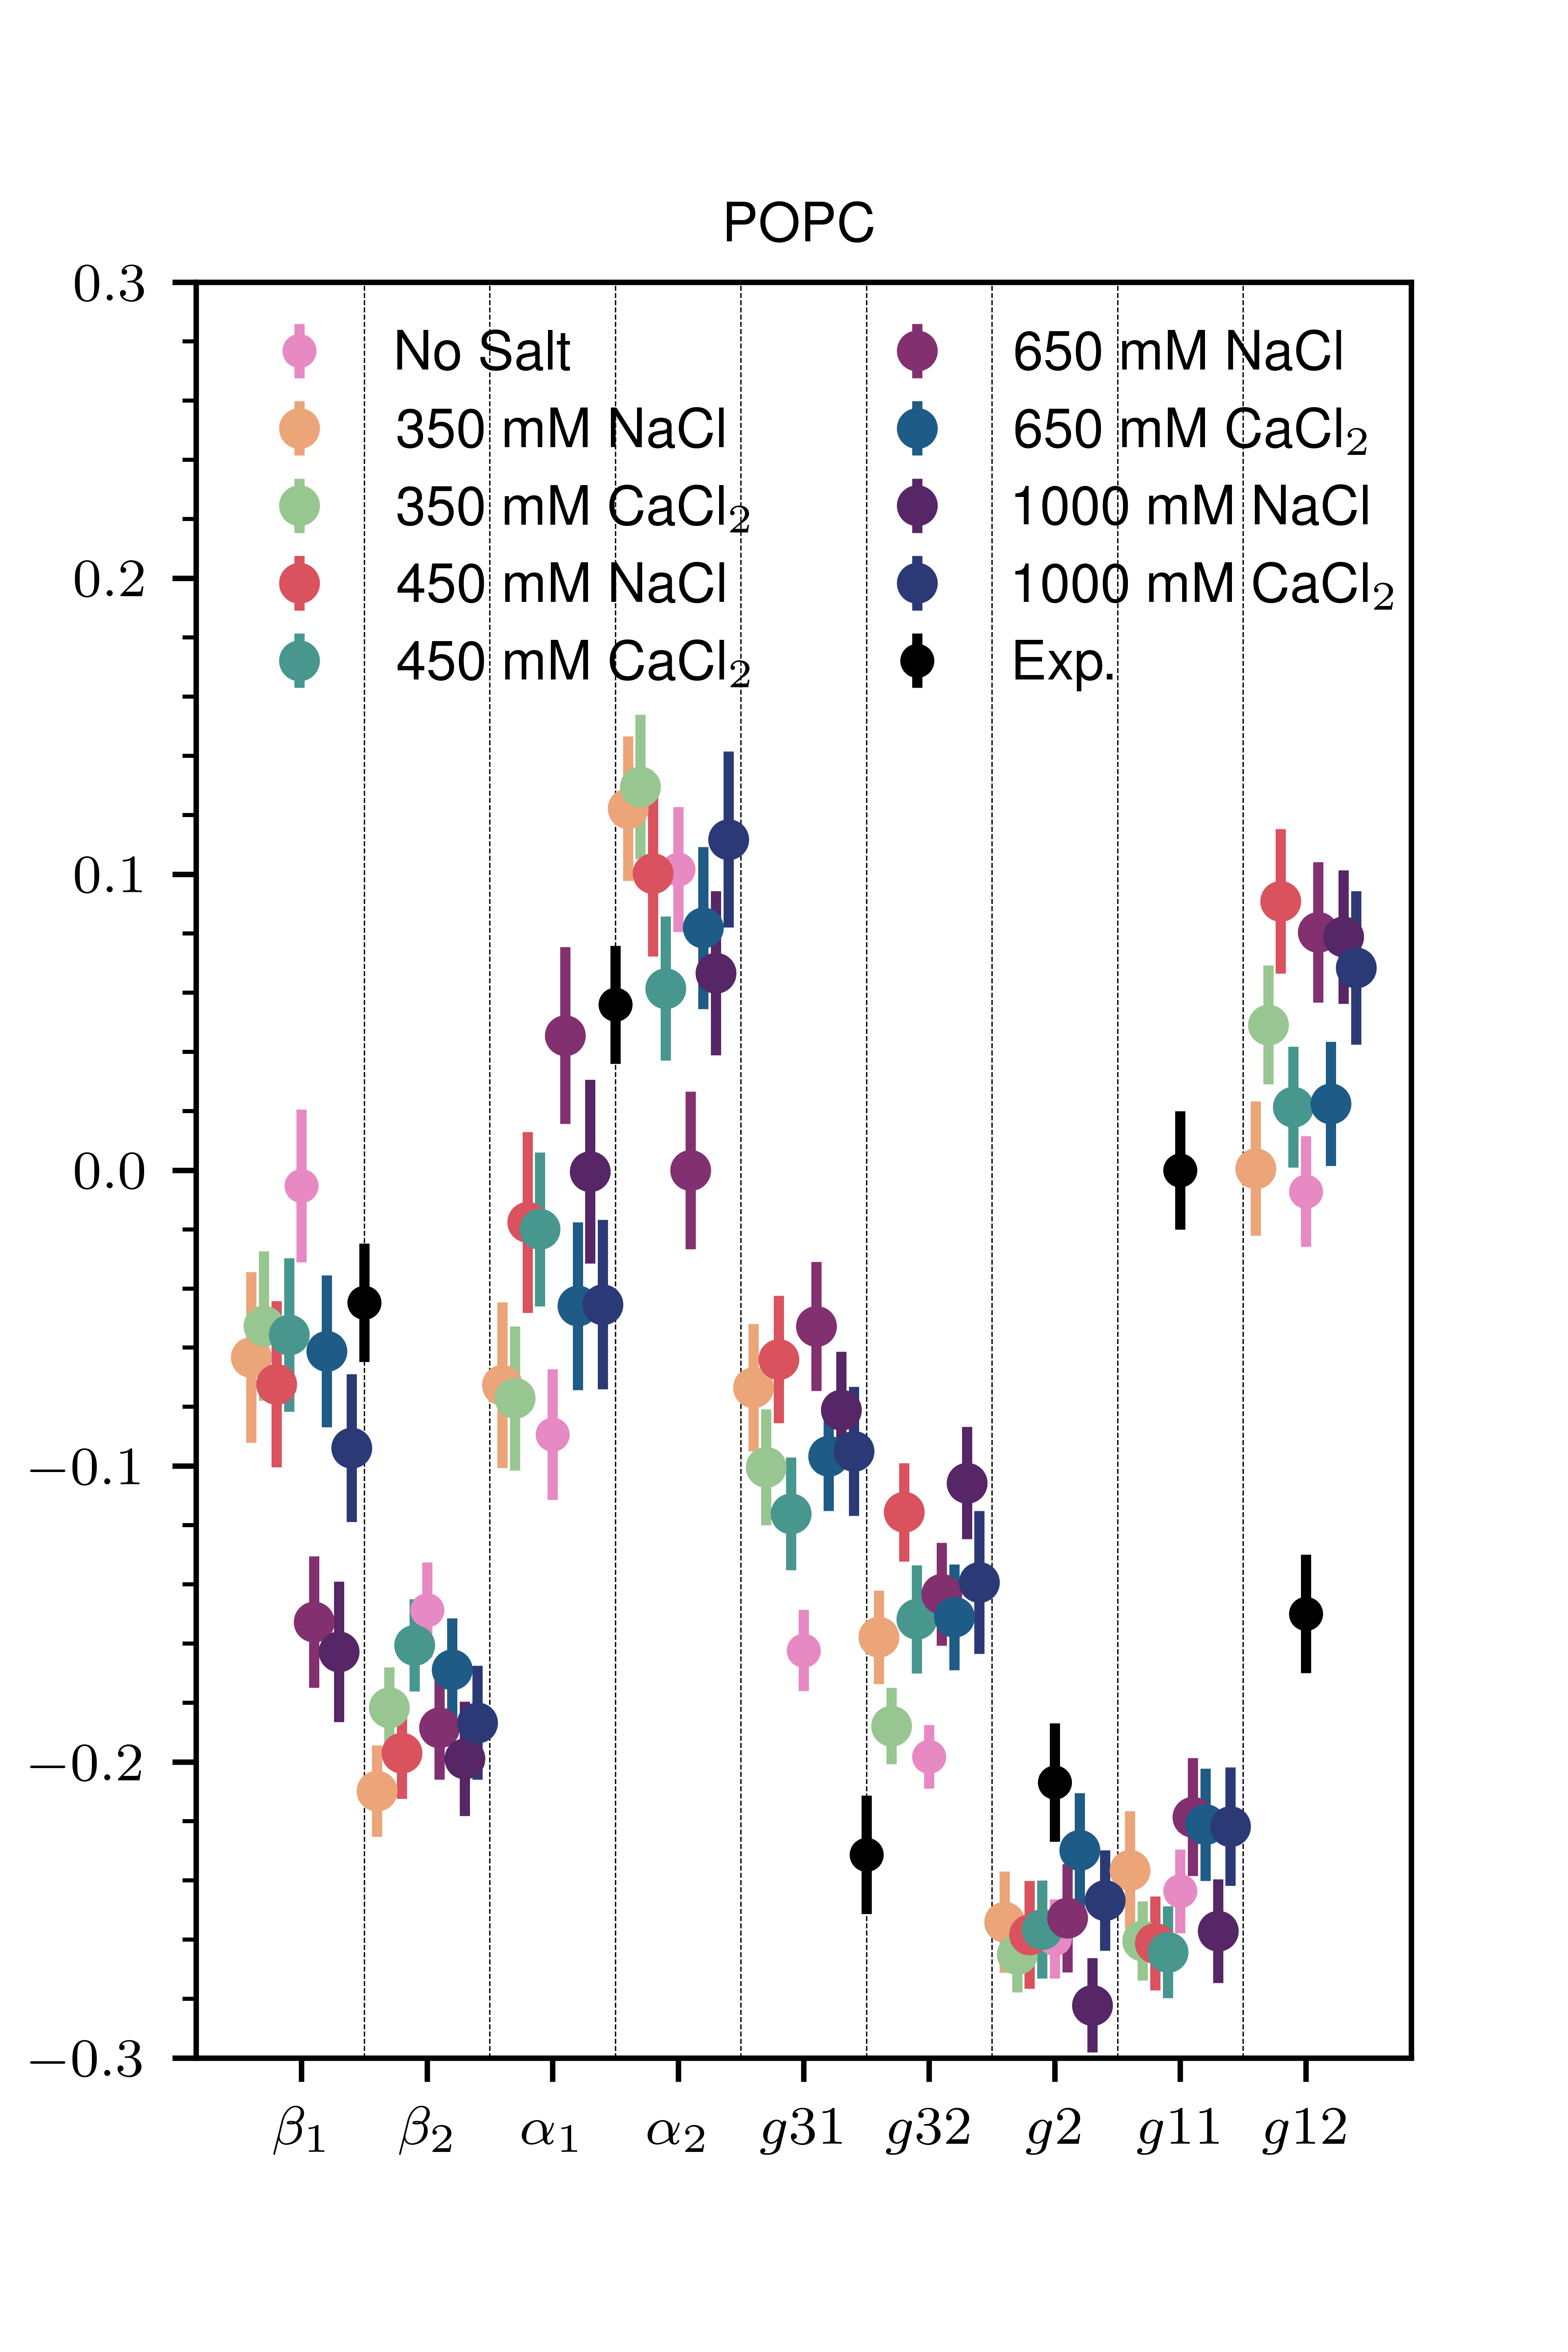
\includegraphics{popc_order_parameters_for_all.png}
%	\caption{The head group and glycerol backbone order parameters $S_{CH}$ for the POPC simulations. The experimental values on the dashed lines mean that the different isomers 1/2 experimentally could not be resolved.}
%	\label{fig:popc_order}
%        \todo{SAMULI: I am not sure if we need this kind of figure. Systems without ions are in separate figures as well as dependence on ions.}
%\end{figure}


\begin{figure}[!hbt]
	\centering
	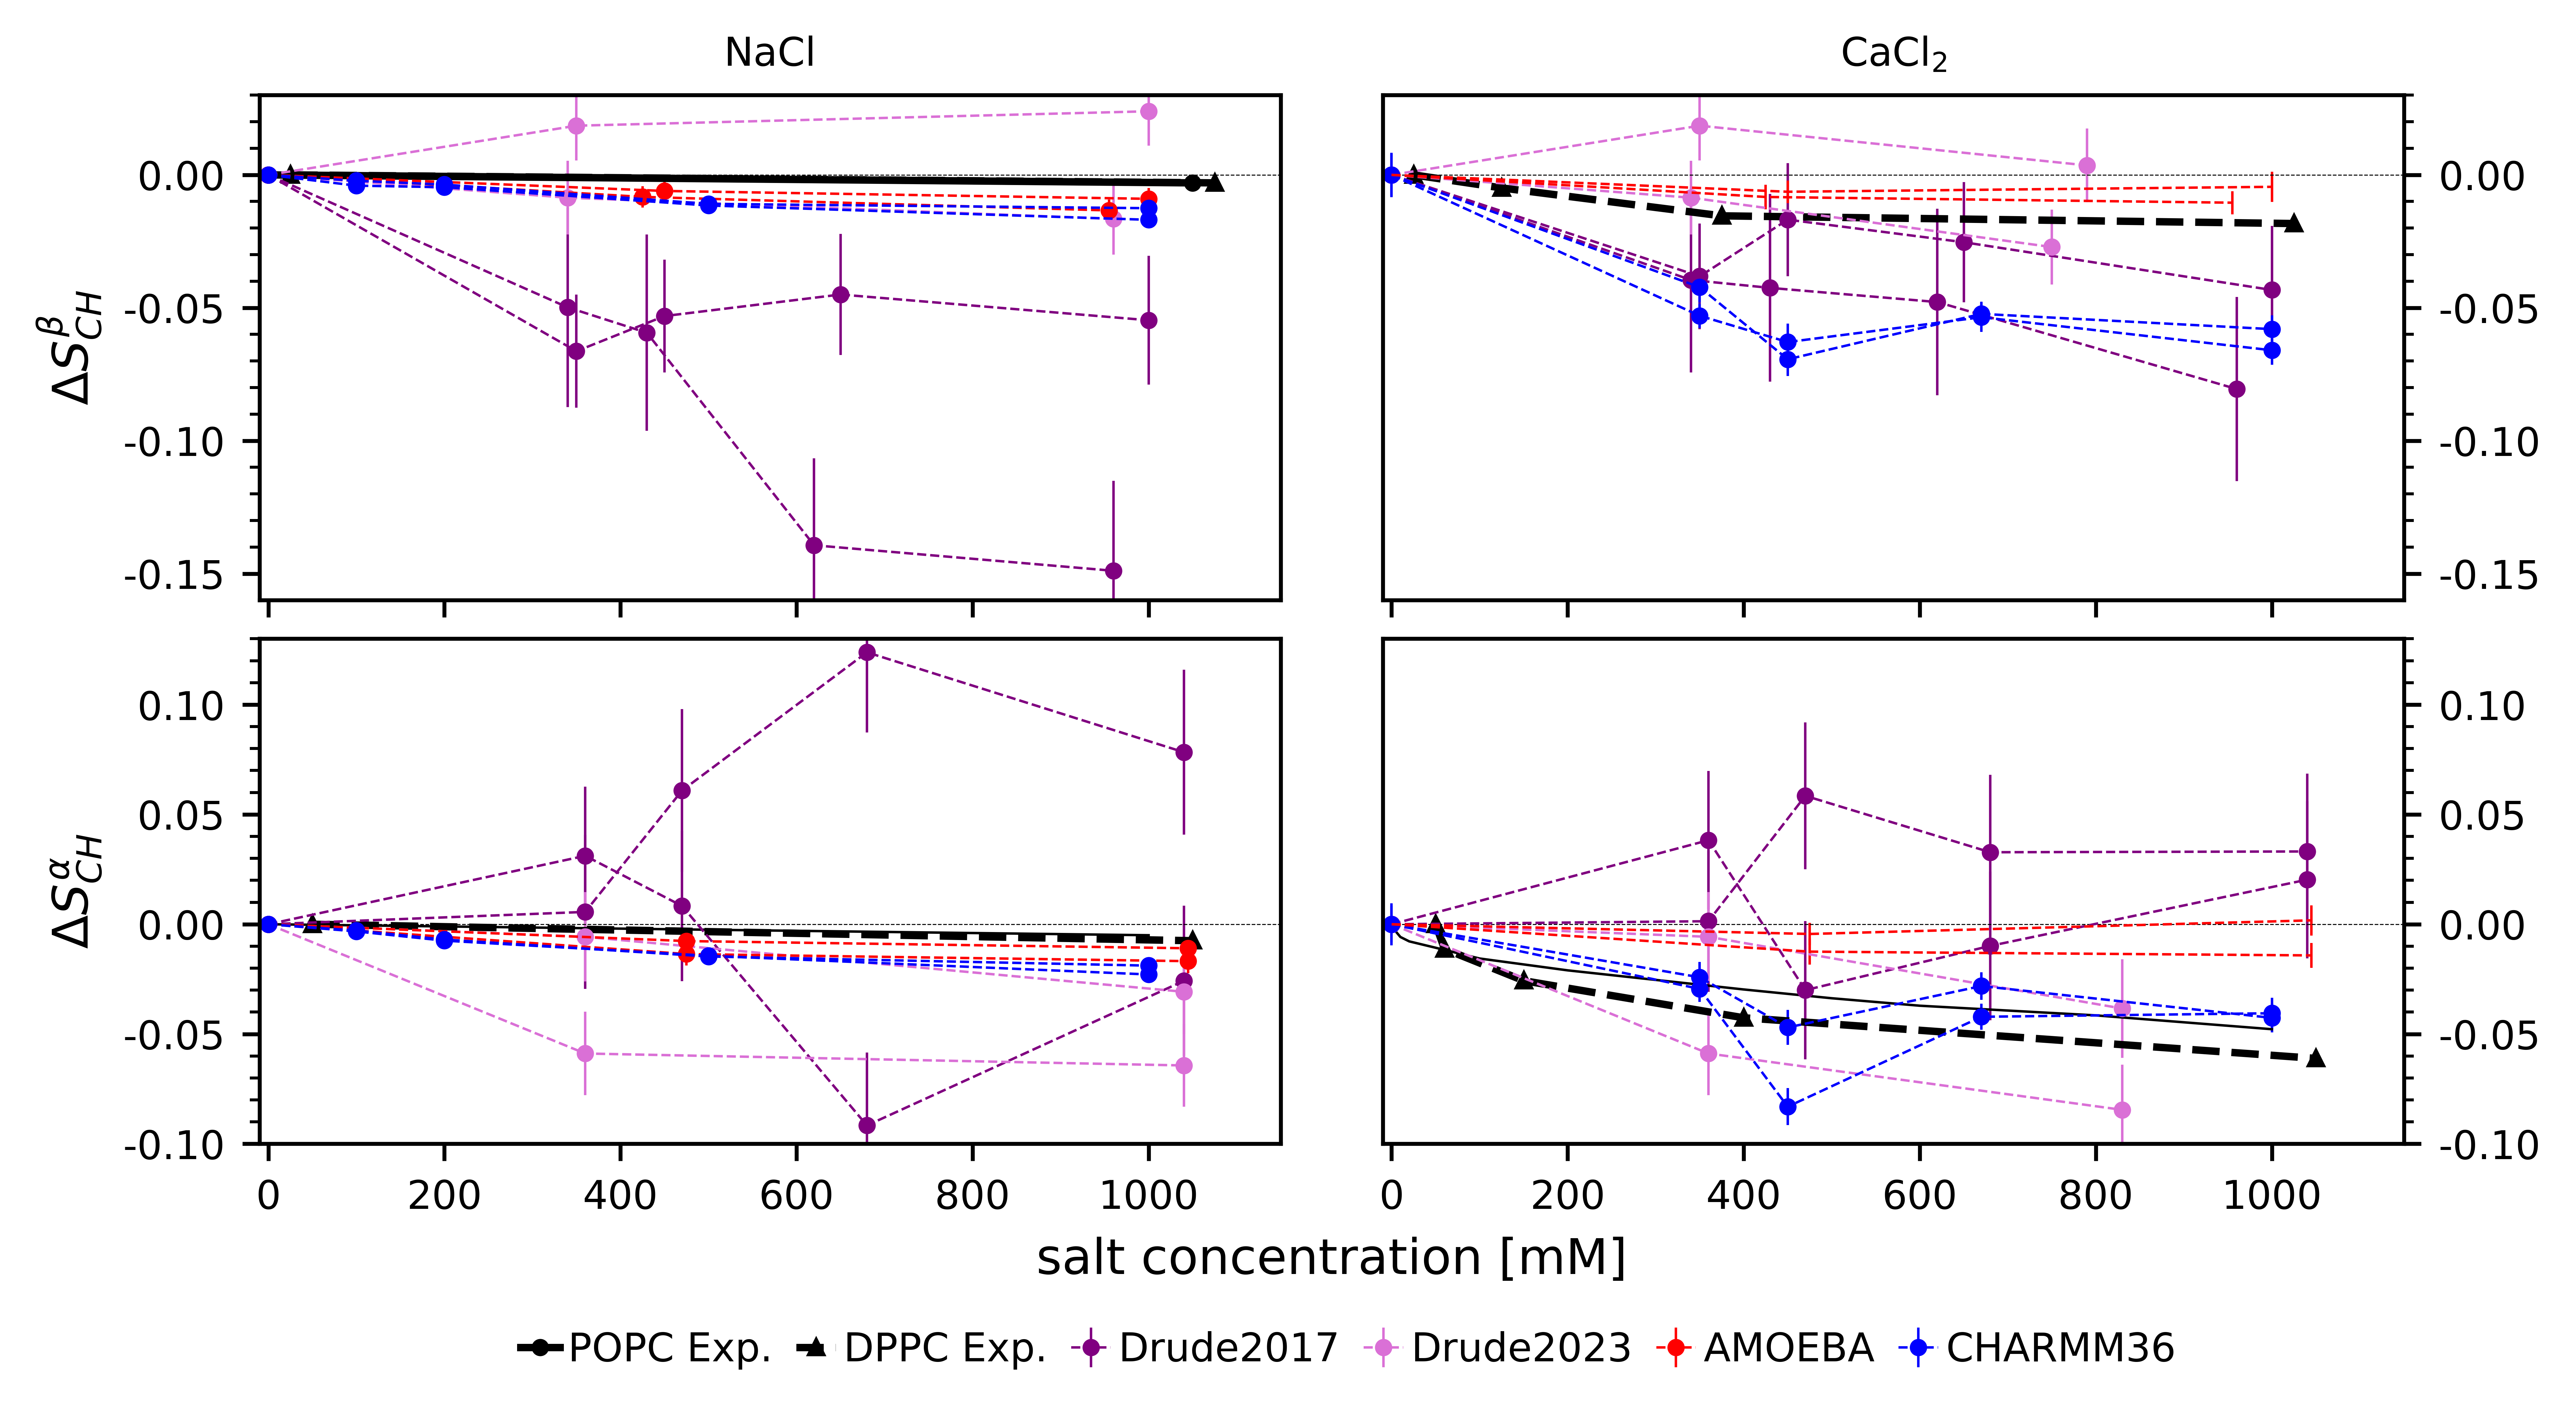
\includegraphics{Figures/order_parameter_change.png}
	\caption{The change in the head group order parameters with respect to the simulations without salt as a function of the salt concentration.}
	\label{fig:popc_order_parameter_change}
        \todo{SAMULI: y-axis scale should be much more zoomed in here, particularly the difference in experiments between sodium and calcium must be visible.} \\
        \todo{SAMULI: We should also show the ion density profiles along membrane normal and compare the ones with 1000 mM NaCl and 350 mM CaCl$_2$
          (concentration in bulk water) to the best profiles in the literature (Fig. 5 in http://dx.doi.org/10.1021/acs.jpcb.7b12510).
          This will show the actual difference in ion binding to the best performing models available.}
\end{figure}

\begin{figure}[!hbt]
    \centering
    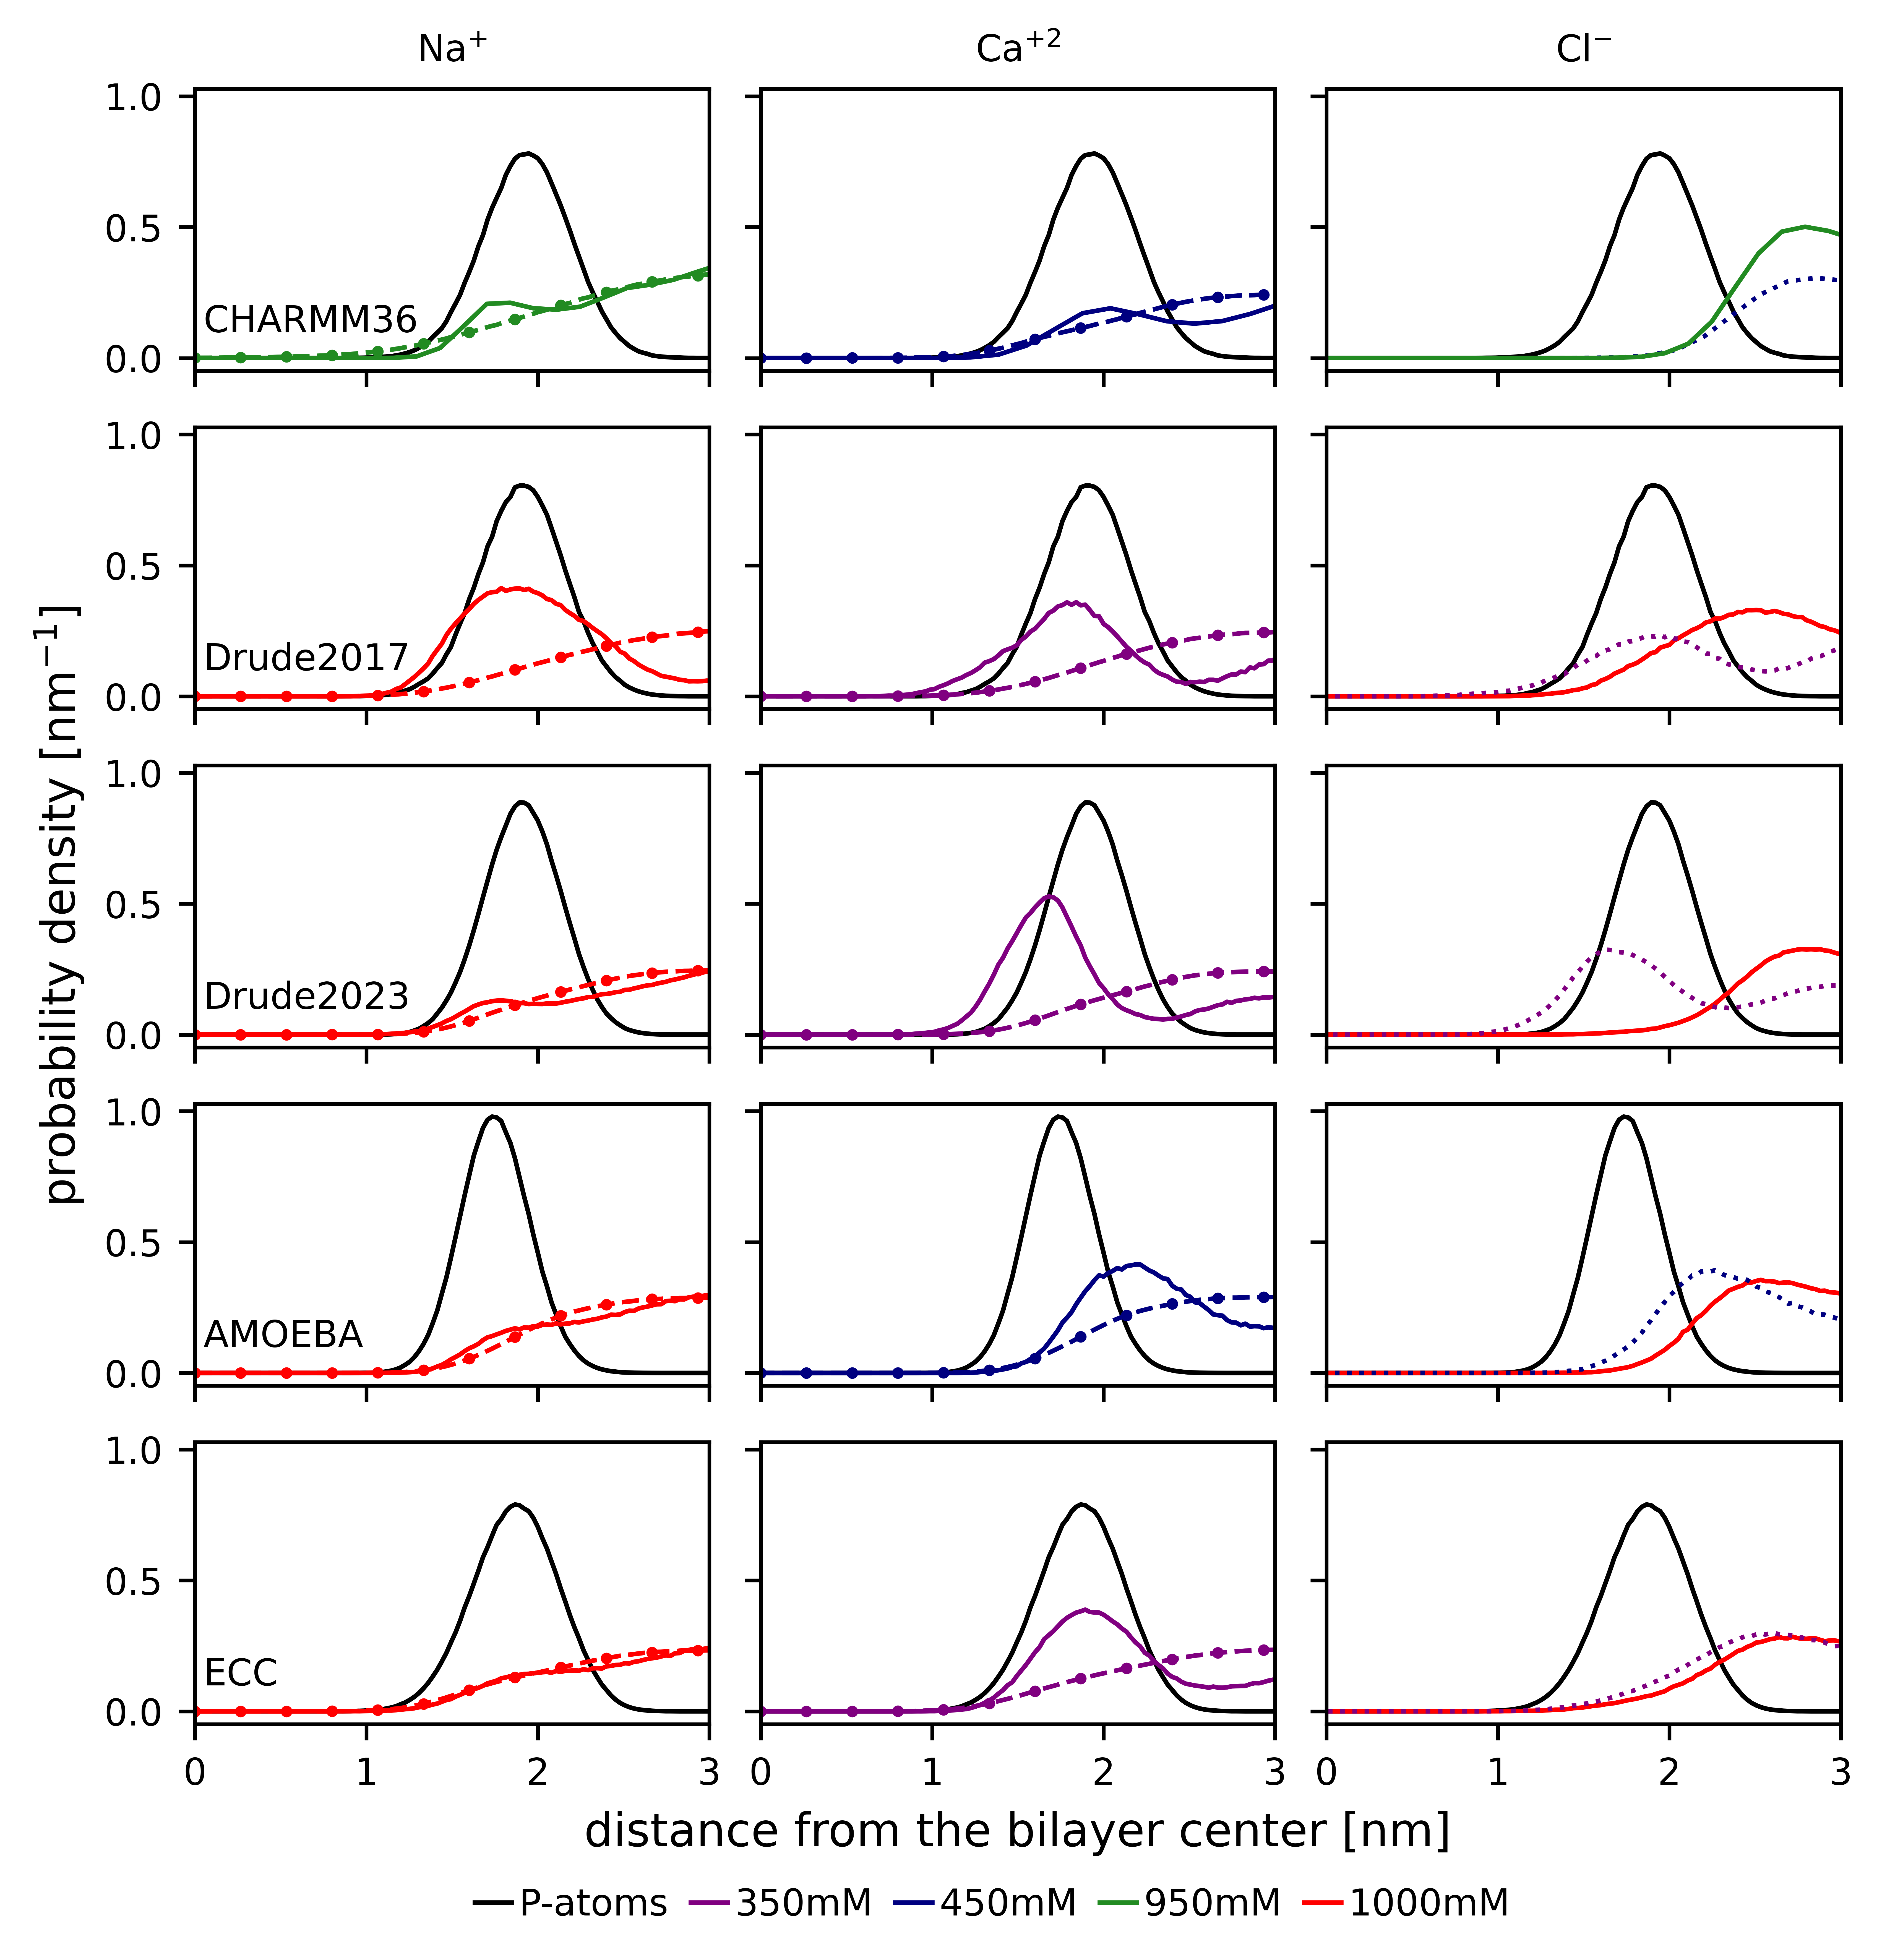
\includegraphics{Figures/ion_density_profiles_with_chloride.png}
    \caption{Density profiles alongside the membrane normal for the Drude POPC (first row) and AMOEBA DOPC (second row). Solid and dashed lines are for the systems with the NaCl and CaCl$_{2}$, respectively.}
    \label{fig:ion_density_profiles}
\end{figure}


\clearpage

\subsection{Discussion}

\subsection{Conclusions}

%%%%%%%%%%%%%%%%%%%%%%%%%%%%%%%%%%%%%%%%%%%%%%%%%%%%%%%%%%%%%%%%%%%%%
%% The "Acknowledgement" section can be given in all manuscript
%% classes.  This should be given within the "acknowledgement"
%% environment, which will make the correct section or running title.
%%%%%%%%%%%%%%%%%%%%%%%%%%%%%%%%%%%%%%%%%%%%%%%%%%%%%%%%%%%%%%%%%%%%%
\begin{acknowledgement}


\end{acknowledgement}

%%%%%%%%%%%%%%%%%%%%%%%%%%%%%%%%%%%%%%%%%%%%%%%%%%%%%%%%%%%%%%%%%%%%%
%% The same is true for Supporting Information, which should use the
%% suppinfo environment.
%%%%%%%%%%%%%%%%%%%%%%%%%%%%%%%%%%%%%%%%%%%%%%%%%%%%%%%%%%%%%%%%%%%%%
\begin{suppinfo}
\end{suppinfo}

%%%%%%%%%%%%%%%%%%%%%%%%%%%%%%%%%%%%%%%%%%%%%%%%%%%%%%%%%%%%%%%%%%%%%
%% The appropriate \bibliography command should be placed here.
%% Notice that the class file automatically sets \bibliographystyle
%% and also names the section correctly.
%%%%%%%%%%%%%%%%%%%%%%%%%%%%%%%%%%%%%%%%%%%%%%%%%%%%%%%%%%%%%%%%%%%%%
\bibliography{nmrlipidsPOL.bib,references.bib}

\end{document}
